\documentclass[11pt,a4paper,roman]{scrartcl}
\usepackage{parskip}
\usepackage[english]{babel}
\usepackage{url}
\usepackage[utf8x]{inputenc}
\usepackage{amsmath}
\usepackage{amssymb}
\usepackage{graphicx}
\usepackage[export]{adjustbox}
\usepackage{listings}
\usepackage{float}
\usepackage{hyperref}
\usepackage[document]{ragged2e}
\usepackage{bm}
\usepackage[section]{placeins}
\title{Computer exercise 3}
\date{}
\author{Carl Ridnert, 940325-0112, ridnert@kth.se \\
Yue Jiao, 911024-7799, yj@kth.se}


\begin{document}
\maketitle
\begin{figure}[h]
\centering
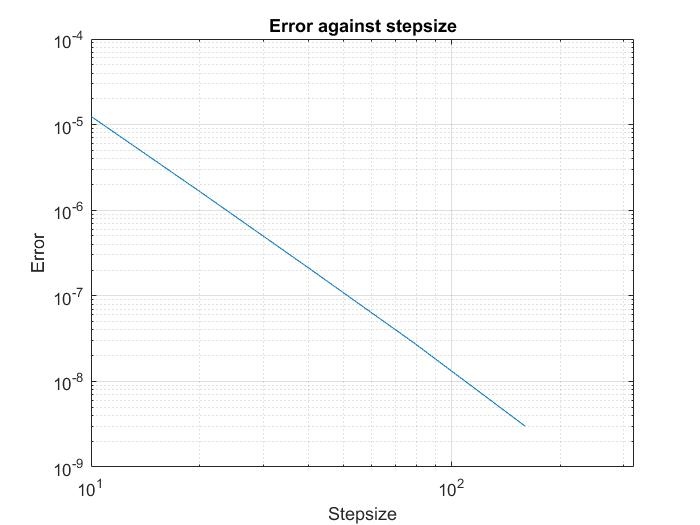
\includegraphics[width=0.45\textwidth,center]{1}
\end{figure}
\newpage

\section*{Solution}
The following problem shall be solved. 
\begin{equation}
-\frac{d}{dz}\left(k\frac{dT}{dz}\right)+\nu \rho C \frac{dT}{dz} = Q(z)
=
\begin{cases} 
      0 & 0\leq z\leq a \\
      Q_0 \cdot sin(\frac{z-a}{b-a}\pi) & a\leq z\leq b \\
      0 & b\leq x \leq L
   \end{cases}
\end{equation}
With the boundary conditions. 
\begin{equation}
\begin{aligned}
T(0) & =T_0 \\ -\kappa \frac{dT}{dz}(L) & = k(T(L)-T_{out})
\end{aligned}
\end{equation}

To solve this equation, the equation is discretized into $N+1$ uniform cells with size $h$. So $(N+1)h=L$. Let $u_i = T(x_i)$ where $x_i = ih$. Since the boundary condition at $T(L)$ is a Robin's condition, a ghost point is added at $L+h$ as $u_{N+1}=L+h$ so that an approximation of second order can be used. \\

Thus the differential equation (1) can be discretized using second order approximations of the derivatives: 
\begin{equation}
-\frac{1}{h}(\kappa\frac{u_{i+1}-u_{i}}{h}-\kappa\frac{u_{i}-u_{i-1}}{h}) + \nu\rho C \frac{u_{i+1}-u_{i-1}}{2h} = Q(x_i) \qquad  \Rightarrow
\end{equation}
\begin{equation}
(-\frac{\kappa}{h^2}+\frac{\nu\rho C}{2h})u_{i+1} + \frac{2\kappa}{h^2}u_i + (-\frac{\kappa}{h^2}-\frac{\nu\rho C}{2h})u_{i-1} = Q(x_i), \qquad i\in[1, 2, ..., N]
\end{equation}

This gives a total of N equations and N+2 unknowns. 

The boundary condition are discretized using second order approximations and gives the two extra equations needed to solve the linear system of equations.
\begin{equation}
\begin{aligned}
u_0 & = T_0 \\ 
-\kappa\frac{u_{N+1}-u_{N-1}}{2h} & = k(u_N-T_{out}) \\ & \Downarrow \\
u_{N+1}+\left(\frac{2hk}{\kappa}\right)u_N - u_{N-1} & = \frac{2hkT_{out}}{\kappa}
\end{aligned}
\end{equation}




A plot of the solutions to the equation system defined by (4) together with the boundary conditions (5) for $\nu=0$ when the number of grid points are varied is shown below. Note that the solutions seems to be converging as the number of points is increased.
\begin{figure}[H]
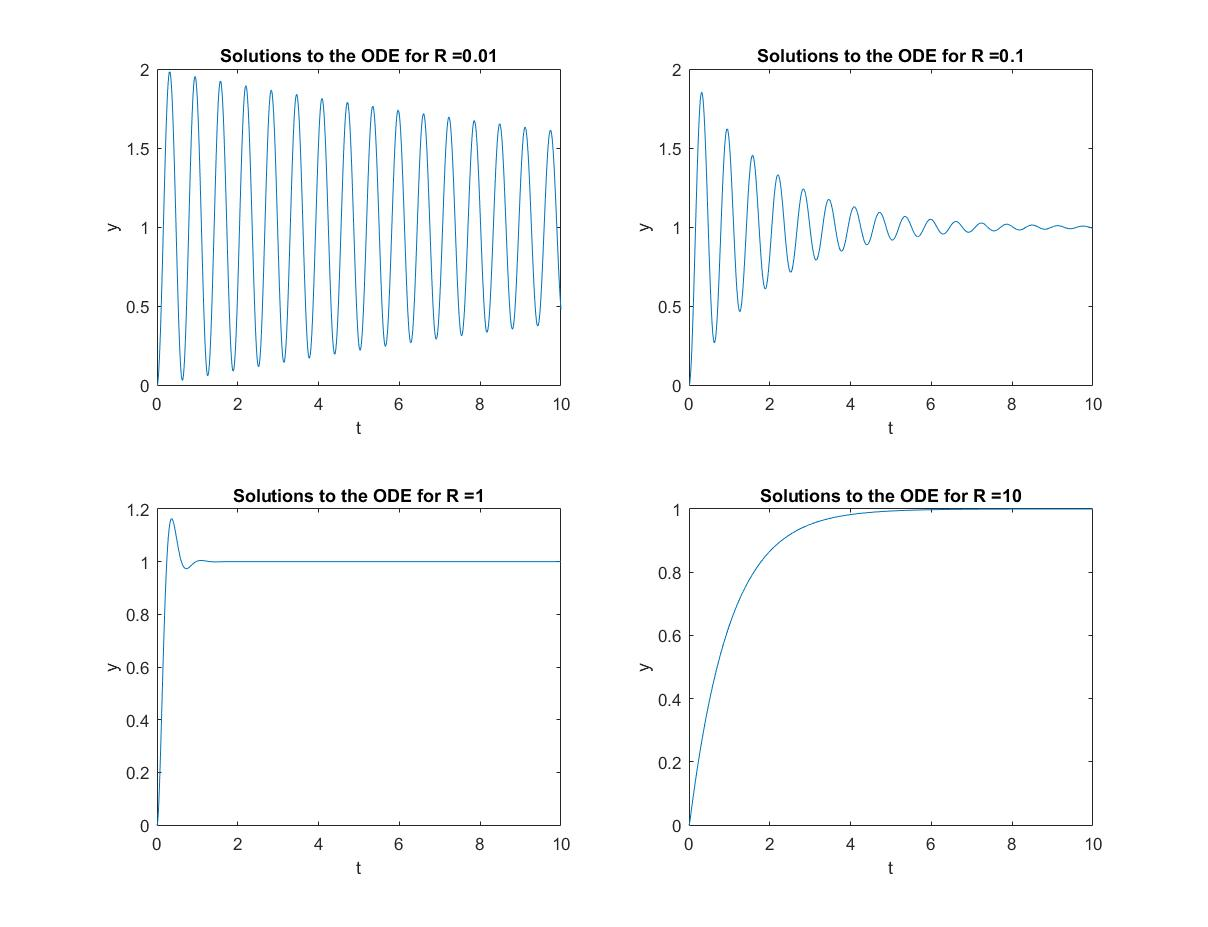
\includegraphics[width=0.7\textwidth,center]{p1}
\caption{Plot with different stepsizes when $\nu = 0$}
\end{figure}

The results were calculated for different $\nu$ with $N=40$ and are showed below. 
\begin{figure}[H]
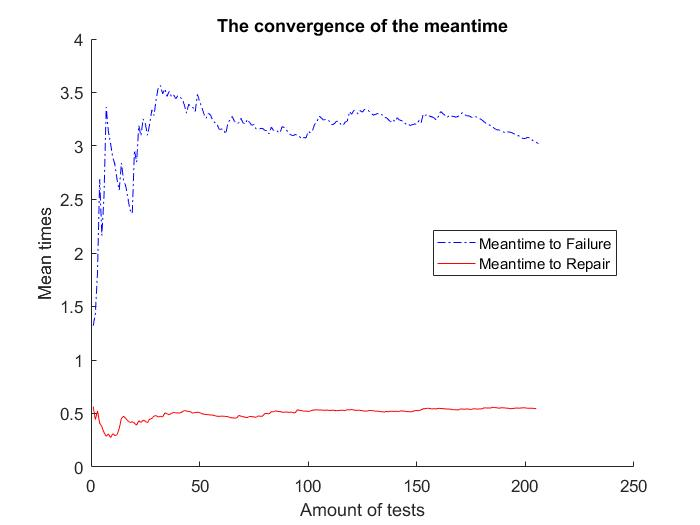
\includegraphics[width=0.7\textwidth,center]{p2}
\caption{Plot with different $\nu$ when $N = 40$}
\end{figure}



It can be observed that the solution of when $\nu = 10$ seems to be oscillating. For a increase in the number of cells N (corresponding to a decrease in the step size h), the oscillations seem to be decreasing as seen in figure 3. 

\begin{figure}[H]
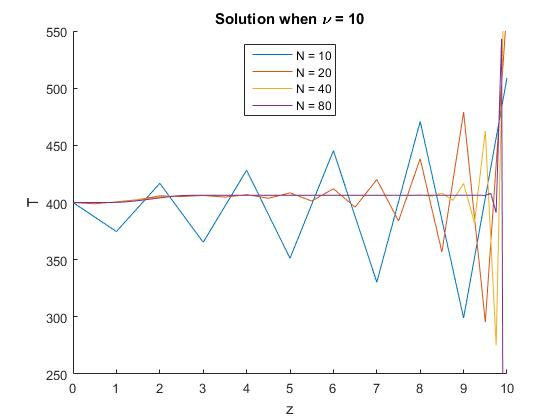
\includegraphics[width=0.7\textwidth,center]{solnu10}
\caption{Plot with different stepsizes when $\nu = 10$}
\end{figure}

The oscillations can be removed by expressing the first derivative in the differential equation through backward Euler's method. This means however that the error becomes of first order instead.
\begin{equation}
\begin{aligned}
-\frac{d}{dz}(k\frac{dT}{dz})+\nu \rho C \frac{dT}{dz} & = Q(z) \\ & \Downarrow \\
-\frac{1}{h}\left(\kappa\frac{u_{i+1}-u_{i}}{h}-\kappa\frac{u_{i}-u_{i-1}}{h}\right) + \nu\rho C \frac{u_{i}-u_{i-1}}{h} & = Q(x_i) \\ & \Downarrow \\
-\frac{\kappa}{h^2}u_{i+1} + \left(\frac{2\kappa}{h^2}+\frac{\nu\rho C}{h}\right)u_i + \left(-\frac{\kappa}{h^2}-\frac{\nu\rho C}{h}\right)u_{i-1}  & = Q(x_i)
\end{aligned}
\end{equation}

By comparison of figure 4 to figure 3, it is clearly visible that the oscillations are removed using the backward Euler method.


\begin{figure}[H]
\centering
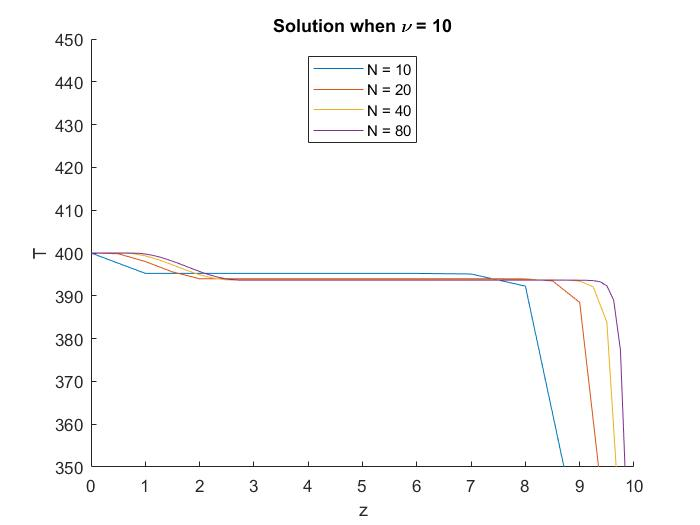
\includegraphics[width=0.7\textwidth,center]{p3}
\caption{Plot for different N when $\nu = 10$}using backward Euler.
\end{figure}

\end{document}

%%%kod

%% Initialization
clear, clc

%% Different stepsize when nu = 0
L = 10; 
a = 1; 
b = 3;
Q0 = 50;
kappa = 0.5;
k = 10;
rho = 1;
C = 1;
Tout = 300;
T0 = 400;
nu = 0;
figure();
hold on;
for N = [10 20 40 80]
    h = L/N;
    N = N+1;
    A = zeros(N);
    bvec = zeros(N,1);
    for i=2:N-1
        A(i,i-1) = -nu*rho*C/2/h-kappa/h^2;
        A(i,i) = 2*kappa/h^2;
        A(i,i+1) = nu*rho*C/2/h-kappa/h^2;
        bvec(i) = Qfunc(i*h, a, b, Q0);
    end
    A(1, 1) = 1;
    A(N, N-2) = -1;
    A(N, N-1) = 2*h*k/kappa;
    A(N, N) = 1;
    bvec(N) = 2*h*k*Tout/kappa;
    bvec(1) = T0;
    T = sparse(A)\bvec;
    plot([0 h*(1:N-1)], [T])
    axis([0, L, 150 450]);
end
title('Solution when \nu = 0')
xlabel('z')
ylabel('T')
legend('N = 10', 'N = 20', 'N = 40','N = 80', 'Location', 'North')

%% Different nu when N = 40
L = 10; 
a = 1; 
b = 3;
Q0 = 50;
kappa = 0.5;
k = 10;
rho = 1;
C = 1;
Tout = 300;
T0 = 400;
N = 40;
figure();
hold on;
for nu = [0 0.1 0.5 1 10]
    h = L/N;
    N = N+1;
    A = zeros(N);
    bvec = zeros(N,1);
    for i=2:N-1
        A(i,i-1) = -nu*rho*C/2/h-kappa/h^2;
        A(i,i) = 2*kappa/h^2;
        A(i,i+1) = nu*rho*C/2/h-kappa/h^2;
        bvec(i) = Qfunc(i*h, a, b, Q0);
    end
    A(1, 1) = 1;
    A(N, N-2) = -1;
    A(N, N-1) = 2*h*k/kappa;
    A(N, N) = 1;
    bvec(N) = 2*h*k*Tout/kappa;
    bvec(1) = T0;
    T = sparse(A)\bvec;
    plot([0 h*(1:N-1)], [T])
    axis([0, L, 150 450]);
end
title('Solution when N = 40 with different \nu')
xlabel('z')
ylabel('T')
legend('\nu = 0', '\nu = 0.1', '\nu = 0.5','\nu = 1', '\nu = 10', 'Location', 'Southeast')

%% Fix spurious
L = 10; 
a = 1; 
b = 3;
Q0 = 50;
kappa = 0.5;
k = 10;
rho = 1;
C = 1;
Tout = 300;
T0 = 400;
nu = 10;
figure();
hold on;
for N = [10 20 40 80]
    h = L/N;
    N = N+1;
    A = zeros(N);
    bvec = zeros(N,1);
    for i=2:N-1
        A(i,i-1) = -kappa/h^2-nu*rho*C/h;
        A(i,i) = 2*kappa/h^2+nu*rho*C/h;
        A(i,i+1) = -kappa/h^2;
        bvec(i) = Qfunc(i*h, a, b, Q0);
    end
    A(1, 1) = 1;
    A(N, N-2) = -1;
    A(N, N-1) = 2*h*k/kappa;
    A(N, N) = 1;
    bvec(N) = 2*h*k*Tout/kappa;
    bvec(1) = T0;
    T = sparse(A)\bvec;
    plot([0 h*(1:N-1)], [T])
    axis([0, L, 350 450]);
end
title('Solution when \nu = 10')
xlabel('z')
ylabel('T')
legend('N = 10', 'N = 20', 'N = 40','N = 80', 'Location', 'North')
    